% ****** Start of file apssamp.tex ******
%
%   This file is part of the APS files in the REVTeX 4.1 distribution.
%   Version 4.1r of REVTeX, August 2010
%
%   Copyright (c) 2009, 2010 The American Physical Society.
%
%   See the REVTeX 4 README file for restrictions and more information.
%
% TeX'ing this file requires that you have AMS-LaTeX 2.0 installed
% as well as the rest of the prerequisites for REVTeX 4.1
%
% See the REVTeX 4 README file
% It also requires running BibTeX. The commands are as follows:
%
%  1)  latex apssamp.tex
%  2)  bibtex apssamp
%  3)  latex apssamp.tex
%  4)  latex apssamp.tex
%
\documentclass[%
 reprint,
%superscriptaddress,
%groupedaddress,
%unsortedaddress,
%runinaddress,
%frontmatterverbose, 
%preprint,
%showpacs,preprintnumbers,
%nofootinbib,
%nobibnotes,
%bibnotes,
 amsmath,amssymb,
 aps,
%pra,
prb,
%rmp,
%prstab,
%prstper,
floatfix,
]{revtex4-1}
 
\usepackage{graphicx}
\usepackage{enumerate}
\usepackage[utf8]{inputenc}
\usepackage{xcolor}
\usepackage{hyperref}
\usepackage{subfig}
\usepackage{floatrow}

\usepackage{amsmath}
\usepackage{amssymb}
\usepackage{arydshln}

\usepackage{tikz}
\usetikzlibrary{positioning,arrows,decorations.markings}

\newcommand{\tjzm}{$t$-$J^z$~model}
\newcommand{\ket}[1]{\left\vert #1 \right\rangle}
\newcommand{\bra}[1]{\left\langle #1 \right\vert}
\newcommand{\abs}[1]{\left\vert #1 \right\vert}

\def\K{%
    \operatornamewithlimits{%
        \mathchoice{% * Display style
            \vcenter{\hbox{\huge $\mathcal{K}$}}%
        }{%           * Text style
            \vcenter{\hbox{\Large $\mathcal{K}$}}%
        }{%           * Script style
            \mathrm{\mathcal{K}}%
        }{%           * Script script style
            \mathrm{\mathcal{K}}%
        }
    }
}

\def\composition{\operatornamewithlimits{\circ}}

\providecommand{\newoperator}[3]{%
	\newcommand*{#1}{\mathop{#2}#3}}
\providecommand{\renewoperator}[3]{%
	\renewcommand*{#1}{\mathop{#2}#3}}
	
\newoperator{\srot}%
	{\mathrm{rot}}{\nolimits}

\newoperator{\ent}%
	{\mathrm{ent}}{\nolimits}
	
\renewoperator{\Re}%
	{\mathrm{Re}}{\nolimits}
	
\renewoperator{\Im}%
	{\mathrm{Im}}{\nolimits}	
	
\makeatletter
\providecommand*{\diff}%
	{\@ifnextchar^{\DIfF}{\DIfF^{}}}
	
\def\DIfF^#1{%
	\mathop{\mathrm{\mathstrut d}}%
	\nolimits^{#1}\gobblespace}
	
\def\gobblespace{%
	\futurelet\diffarg\opspace}
	
\def\opspace{%
	\let\DiffSpace\!%
		\ifx\diffarg(%
			\let\DiffSpace\relax
		\else
			\ifx\diffarg[%
				\let\DiffSpace\relax
			\else
				\ifx\diffarg\{%
					\let\DiffSpace\relax
				\fi\fi\fi\DiffSpace}
				
\providecommand*{\deriv}[3][]{%
	\frac{\diff^{#1}#2}{\diff #3^{#1}}}
\providecommand*{\pderiv}[3][]{%
	\frac{\partial^{#1}#2}%
		{\partial #3^{#1}}}
		
\newcommand{\mean}[1]{\langle#1\rangle}

\begin{document}

\title{Title?}

%\title{Magnon-magnon Interaction Induced Incoherence in the 2D  Doped Antiferromagnets}% Force line breaks with \\
%\thanks{A footnote to the article title}%

\author{Piotr Wrzosek$^1$}
\author{Krzysztof Wohlfeld$^1$}
\author{Eugene Demler$^{2,3}$}
\author{Annabelle Bohrdt$^{3,4}$}
\author{Fabian Grusdt$^{5,6}$}

\affiliation{%
$^1$Institute of Theoretical Physics, Faculty of Physics, University of Warsaw, Pasteura 5, PL-02093 Warsaw, Poland
}%

\affiliation{%
$^2$Institute for Theoretical Physics, ETH Zurich, Zurich, Switzerland
}%

\affiliation{%
$^3$Department of Physics, Harvard University, Cambridge, Massachusetts 02138, USA
}%

\affiliation{%
$^4$ITAMP, Harvard-Smithsonian Center for Astrophysics, Cambridge, MA 02138, USA
}%

\affiliation{%
$^5$Department of Physics and Arnold Sommerfeld Center for Theoretical Physics (ASC),
Ludwig-Maximilians-Universit\"at M\"unchen, Theresienstr. 37, M\"unchen D-80333, Germany
}%

\affiliation{%
$^6$Munich Center for Quantum Science and Technology (MCQST), Schellingstr. 4, D-80799 M\"unchen, Germany
}%


\date{\today}% It is always \today, today,
             %  but any date may be explicitly specified

\begin{abstract}
Abstract...

\end{abstract}

\pacs{Valid PACS appear here}% PACS, the Physics and Astronomy
                             % Classification Scheme.
%\keywords{Suggested keywords}%Use showkeys class option if keyword
                              %display desired
\maketitle

%\tableofcontents

\section{\label{sec:intro}Introduction}

\section{\label{sec:model_methods}Model \& Methods}

Local Greens function with rotational degrees of freedom can be written as
\begin{equation}
    G^{\text{rot}}_{M_n}(\omega) = 
    \bra{0_\sigma}R^{\dag}_{\sigma,M_n}(0) 
        \hat{G}(\omega)
    R_{\sigma,M_n}(0) \ket{0_\sigma}.
\end{equation}
where $\hat{G}(\omega) = (\omega - H + E_0)^{-1}$.  
\begin{align}
	\mathcal{H}_t &= -t\sum_{\mean{ij}\sigma} \tilde{c}_{i\sigma}^\dag \tilde{c}_{j\sigma}
	+ \mathrm{H.c.} \\
	\mathcal{H}_J &= J\sum_{\mean{ij}} \left(S_i^z S_j^z - \frac{1}{4}\tilde{n}_i \tilde{n}_j\right)
\end{align}
$H = \mathcal{H}_t + \mathcal{H}_J$ stands for the \tjzm{} Hamiltonian with the ground state $\ket{0_\sigma}$ in the half-filled limit. We denote energy of $\ket{0_\sigma}$ as $E_0$. The label $\sigma \in \{-1/2, 1/2\}$ stands for the spin at the origin of the lattice, i.e. at site $i = 0$. Double occupancy is projected out, i.e. $\tilde{c}_{i\sigma}^\dag = c_{i\sigma}^\dag (1 - c_{i\bar{\sigma}}^\dag c_{i\bar{\sigma}})$, and $\tilde{n}_i = \sum_{\sigma} \tilde{c}_{i\sigma}^\dag \tilde{c}_{i\sigma}$. Operator $R_{\sigma,M_n}(i)$ removes the electon with spin $\sigma$ from site $i$ and then creates a normalised linear combination of states where the created hole has been propagated exactly $n$ times without returning. With each hop the hole acquires a phase proportional to $M_n(j) = m^{(j)}$, where $M_n = (m^{(1)}, ..., m^{(n)})$ is ordered collection of phase factors.

Within the self-avoiding walks approximation operator $R_{\sigma,M_n}(i)$ is restricted only to paths that do not cross themselves. In the same time, the rotational Greens function can be rewritten in the following form,
\begin{equation}
    G^{\text{rot}}_{M_n}(\omega) = 
    \frac{1}{\abs{\mathcal{A}_n}}\sum_{\eta, \eta' \in \mathcal{A}_n}
	\mathcal{P}_{M_n}^{\eta',\eta}
        %e^{i m(\varphi_\xi - \varphi_{\xi'})}
        G_{\eta', \eta}(\omega),
\end{equation}
where $\ket{\eta}$ and $\ket{\eta'}$ denote states with the hole created at the origin $(i = 0)$ and propagated $n$ times to site $j \neq 0$, such that the hole does not cross its own path. We call this type of the motion of the hole a self-avoiding walk (or self-avoiding path) and denote the set of self-avoiding paths with length $n$ as $\mathcal{A}_n$. We also define the coefficient of the Greens function,
\begin{equation}
    G_{\eta', \eta}(\omega) = \bra{\eta'}\hat{G}(\omega)\ket{\eta},
\end{equation}
and the phase contribution from the angular momentum of the hole is denoted as $\mathcal{P}_{M_n}^{\eta',\eta}$. For details on definition and calculations of $\mathcal{P}_{M_n}^{\eta',\eta}$ have a look at the Appendix~\ref{sec:appendix:phases}. 

The task is to calculate coeffcient $G_{\eta', \eta}(\omega)$ for a given pair of self-avoiding paths $\eta$ and $\eta'$.
Let us denote $\hat{H}(\omega) = (\omega - H + E_0)$ such that $\hat{G}(\omega) = \hat{H}(\omega)^{-1}$. Then let define basis $\mathcal{B}$ of all possible states $\ket{\eta}$ of the system, where there exists $n$ such that $\eta \in \mathcal{A}_n$. In general we can find elements $G_{\eta', \eta}(\omega)$ with cofactor matrix method,
\begin{equation}
    \mathcal{M}(\hat{G}(\omega))_\mathcal{B}^\mathcal{B} = 
    \frac{C^{T}(\omega)}{\det \mathcal{M}(\hat{H}(\omega))_\mathcal{B}^\mathcal{B}},
\end{equation}
where matrix $C = [C_{i,j}]$, coefficients $C_{i,j} = (-1)^{i+j}M_{i,j}$ and $M_{i,j}$ is the $(i,j)$-minor of the matrix $\mathcal{M}(\hat{H}(\omega))_\mathcal{B}^\mathcal{B}$ with $i$-th row and $j$-th column removed. 

Let $\eta_n = \xi_1 \xi_2 \hdots \xi_n$ for $n>0$, where $\xi_j \in D$ denotes $j$-th move of the hole and $\eta_0 = 1$ for $n=0$. On a square lattice (or on the Bethe lattice) with coordination number $z=4$ we can put for example $D = \{E,N,W,S\}$ denoting 4 possible directions of the propagation from each site.

Let us further introduce function $\mathcal{S}$ that takes a self-avoiding path $\eta_n$ of the hole and returns set of moves $\Delta$ leading to the self-avoiding paths $\eta_{n+1} = \eta_n \xi_{n+1}$ reachable from the path $\eta_n$. Then we can write,
\begin{equation}\label{eq:Sigma}
    t^2\Sigma_{\eta_k}(\omega)^{-1} = G_{\eta_k}(\omega)^{-1} - \sum_{\xi \in \mathcal{S}(\eta_k)}\Sigma_{\eta_k \xi}(\omega),
\end{equation}
where
\begin{equation}
    G_{\eta_k}(\omega)^{-1} = 
    \bra{\eta_k}
    \left(
        \omega - \mathcal{H}_J + E_{0}
    \right)
    \ket{\eta_k}.
\end{equation}
Moreover we define,
\begin{equation}\label{eq:Gamma}
    \Gamma_{\eta_k}^{\Delta}(\omega) = G_{\eta_k}(\omega)^{-1} - \sum_{\xi \in \Delta}\Sigma_{\eta_k \xi}(\omega),
\end{equation}
where $\Delta \subset D$. The above defined $\Gamma_\eta^{\Delta}(\omega)$ can be evalueted numerically assuming finite depth of the recursion in the Eq.~\eqref{eq:Sigma}. One can adjust the depth of the recursion to ensure convergence, provided that the value of the coupling constant is not too small, i.e. $J > 0.2t$ for the square lattice or $J > 0.01t$ for the Bethe lattice where symmetry allows for improvements.

In the end, the generic formula for $G_{\eta'_l, \eta_r}(\omega)$ can be found in the following form, 
\begin{equation}\label{eq:GFcoef}
	\begin{split}
		&\bra{\xi'_1 \xi'_2 \hdots \xi'_l}
		\hat{G}(\omega)
		\ket{\xi_1 \xi_2 \hdots \xi_r} = (-t)^{r + l - 2c} \times \\
		&\frac{\displaystyle
		\prod_{k=0}^{c-1} \left(
			\Gamma_{\eta_k}^{\mathcal{S}(\eta_k)\setminus\{\xi_{k+1}\}} - \K_{n=k+1}^{c-1} \frac{t^2}{\Gamma_{\eta_n}^{\mathcal{S}(\eta_n)\setminus\{\xi_{n+1}\}}}
		\right)
		}{\displaystyle
		\left(
			\prod_{k=0}^{c} \Gamma_{\eta_k}^{\mathcal{S}(\eta_k)}
		\right)
		\left(
			\prod_{k=c+1}^{r} \Gamma_{\eta_k}^{\mathcal{S}(\eta_k)}
		\right)
		\left(
			\prod_{k=c+1}^{l} \Gamma_{\eta_k}^{\mathcal{S}(\eta_k)}
		\right)
		},    
	\end{split}
\end{equation}
where we have $\xi'_j = \xi_j$ for all $j \leq c$ and either $c = \min(l,r)$ or $\xi'_{c+1} \neq \xi_{c+1}$. Moreover, to shorten the notation we write $\Gamma_\eta^\Delta \equiv \Gamma_\eta^\Delta(\omega)$. Additionally, we present an intuitive representation of the above equation using simple diagrams in the Appendix~\ref{sec:appendix:diagrams}

\section{\label{sec:results}Results}

\subsection{\label{sec:results:no_rot}Spectral functions without rotations}

We now know how to efficiently calculate off-diagonal coefficients of the Greens function within self-avoiding paths approximation. Therefore we can easily find spectral function of a single hole insert to an Ising antiferromagnet with rotational degrees of freedom. In the discussion below we present results concerning major 4 cases. These cases include choice of the lattice (either square or Bethe) and contribution form magnon-magnon interactios (either included of discarded). Within these cases we have 3 minor cases for distinct rotational degrees of freedom, namely: no rotations, one angular momentum and two angular momenta.

We start with simplest case of a single hole without rotations. Corresponding spectral functions as a function of energy $\omega$ and coupling constant $J$ are presented in Fig.~\ref{fig:no_rot} (with magnon interaction included) and Fig.~\ref{fig:no_rot_no_mag} (without magnon interactions). For each $J$ spectral function is shifted in $\omega$ such that the ground state energy equals 0. In the mentioned figures there is a peak at 0 energy but in general weight at the ground state energy does not have to be finite, what will be visible once we include rotational degrees of freedom.

\begin{figure}[ht!]
	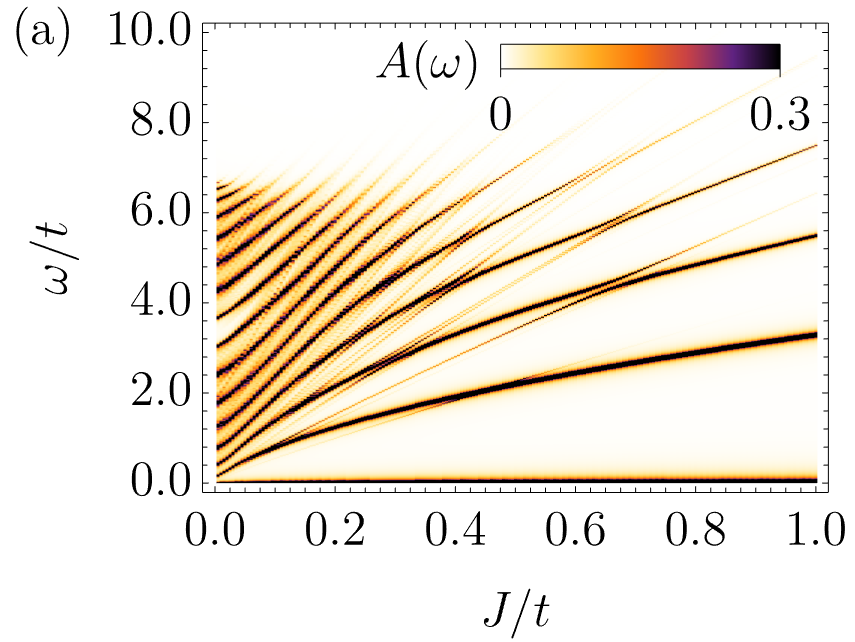
\includegraphics[width=0.49\columnwidth]
	{./figures/square/Int64[]_noint.png}
	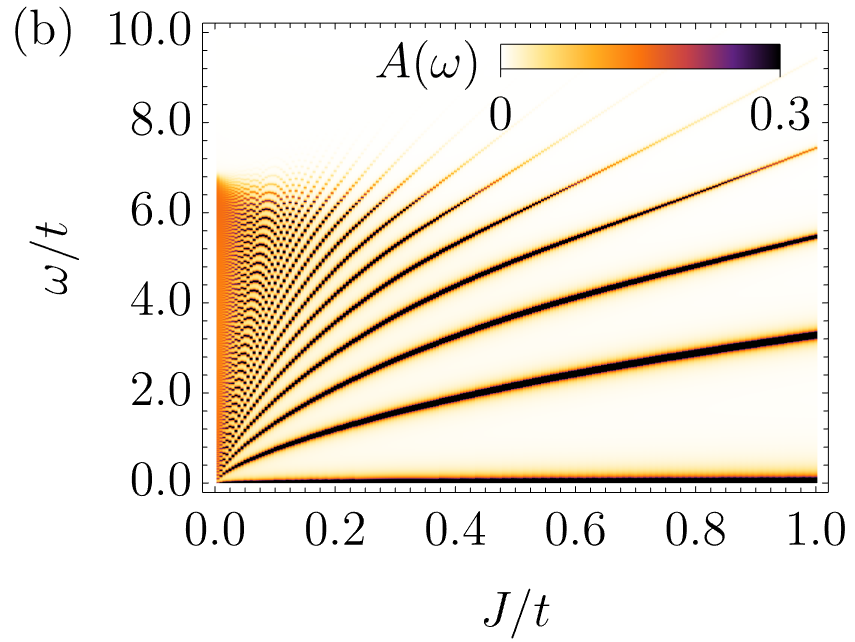
\includegraphics[width=0.49\columnwidth]
	{./figures/bethe/Int64[]_noint.png}
	\caption{
		Spectral function $A(\omega)$ of a singe hole doped to the Ising antiferromagnet calculated within self-avoiding walks approximation without interactions, (a) on the square lattice and (b) on the Bethe lattice. Coupling constant $J=0.4t$.
	}\label{fig:no_rot_no_mag}
\end{figure}

In Fig.~\ref{fig:no_rot_no_mag} we can see a rather subtle but quatitative effect of changing the lattice form Bethe to square. Overall, peaks present in the Bethe lattice are well visible also on the square lattice. Distance between these peaks scale as $(J/t)^{2/3}$. But on the square lattice we can also see additional features. Position of these features scales linearily with $J/t$. Since these features are visible also for large $J/t$ we believe they should not be destroyed by including the hole motion in closed paths. But to fully confirm this claim one should perform exact diagonalisation study on the square lattice without magnon-magnon interactions.

We would also like to draw the attention to the small $J/t$ region. Apparent discrepancy between density of peaks for $J/t < 0.2$ on the square and the Bethe lattices is a false result comming from the limitations of the method. For the Bethe lattice we are able to include chains of up to 1000 magnons in length. But for the square lattice this number is reduced to several (usually slightly less than 20) and this is not enough to obtain converged results for $J/t < 0.3$. In the end, number of peaks we see is too small and in reality it should be much more similar to the case of the Bethe lattice.

\begin{figure}[ht!]
	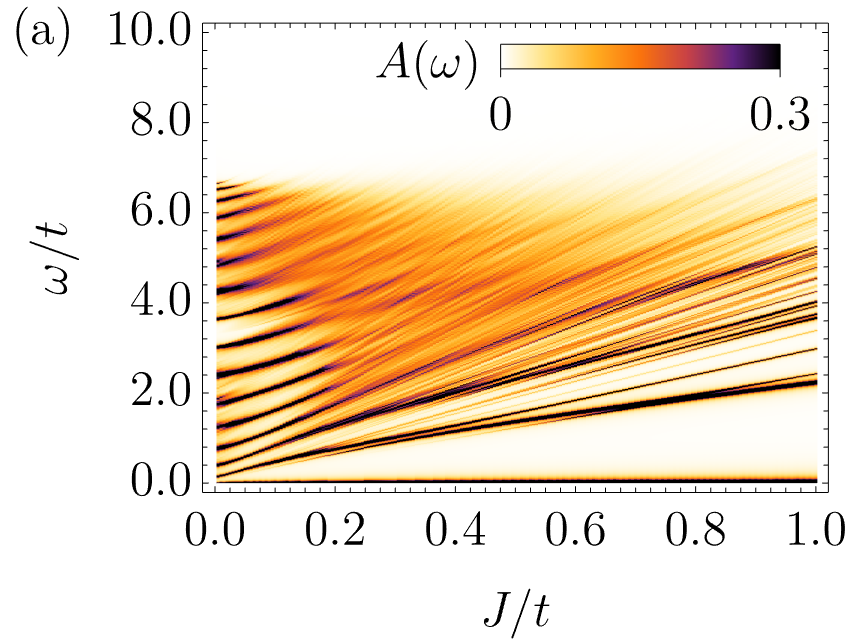
\includegraphics[width=0.49\columnwidth]
	{./figures/square/Int64[].png}
	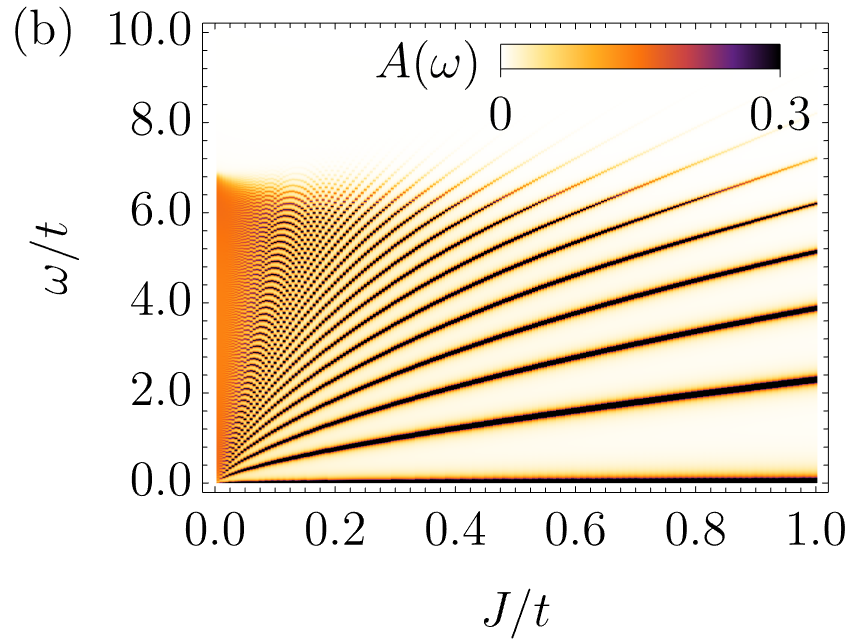
\includegraphics[width=0.49\columnwidth]
	{./figures/bethe/Int64[].png}
	\caption{
		Spectral function $A(\omega)$ of a singe hole doped to the Ising antiferromagnet calculated within self-avoiding walks approximation (with interactions included), (a) on the square lattice and (b) on the Bethe lattice. Coupling constant $J=0.4t$.
	}\label{fig:no_rot}
\end{figure}

Now let us analyze the case with magnon-magnon interactions included. In the Fig.~\ref{fig:no_rot} we see a different effect of magnon interactions, dependent on the lattice. Comparing with Fig.~\ref{fig:no_rot_no_mag} we see that for the Bethe lattice magnon interactions only quantitativle influence the spectral function. Here they merely rescale the distance between the peaks. This result is not surprising and it can be easily explained as showed in previous works \onlinecite{Wrzosek2021}. On the other hand on the square lattice magnon interactions introduce a broad continuum. This result is more subtle and comes from distinct energies of paths with the same number of magnons. Two path with the same number of magnons may have different energy if they become tangential, allowing for additional interactions between the magnons. On the Bethe lattice this is not possible and magnons always interact only along the path of the moving hole. These effect was also studied in details in the prevous work \onlinecite{Bie19,Wrzosek2021}. In the same time one can still see significantly pronouced weight on top of the continuum at the positions corresponding to peaks visible on the Bethe lattice. Moreover, on the square lattice we can see additional peaks, linear in $J/t$, similarily to the result without magnon interactions (cf. Fig.~\ref{fig:no_rot_no_mag}a and Fig.~\ref{fig:no_rot}a). Interrestingly the number of these lines is much higher in case with magnon interactions. This is consistent with understanding of the role of magnon interactions that drives massive spitting of peaks due to different energy cost of paths with the same number of magnons.

\subsection{\label{sec:results:one_rot}Spectral functions with single rotation}

Now let us investigate the spectral function of a single hole with one rotational degree of freedom. Microscopically it corresponds to creating a hole in a given site and then propagating it to nearest sites with phase factor dependent on the direction,
\begin{equation}
	R_{\sigma,M_1}(0) \ket{0_\sigma} = \sum_{\xi \in D} e^{-i m^{(1)} \phi_\xi} \ket{\xi},
\end{equation}
where $D = \{E,N,W,S\}$ and $\phi_\xi \in \{\frac{n\pi}{2}\}_{n\in0...3}$ is given by relation $(E,N,W,S) = (0,1,2,3)$. The only free parameter is a phase factor $m^{(1)} \in \{0,...,3\}$. But for self-avoiding paths approximation there are only two distinct spectral functions -- one for $m^{(1)} = 0$ and the other one for remeaining values.

\begin{figure}[ht!]
	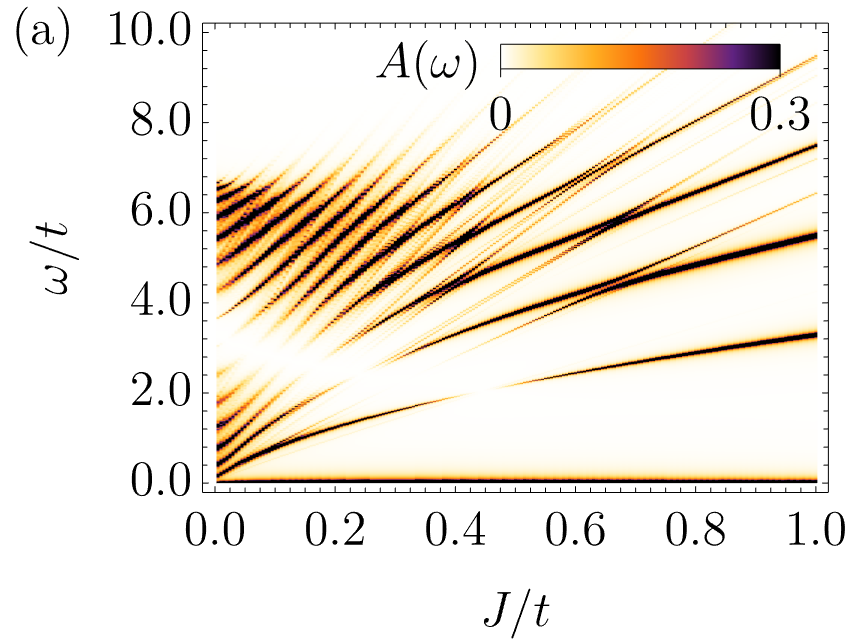
\includegraphics[width=0.49\columnwidth]
	{./figures/square/[0]_noint.png}
	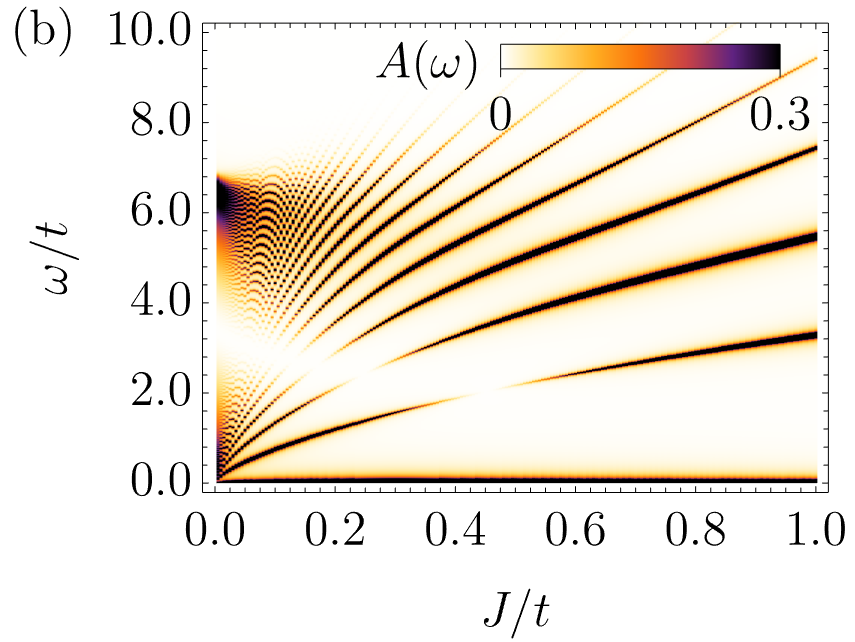
\includegraphics[width=0.49\columnwidth]
	{./figures/bethe/[0]_noint.png}
	\caption{
		Spectral function $A(\omega)$ of a singe hole with rotational degrees of freedom calculated within self-avoiding walks approximation without interactions, (a) on the square lattice and (b) on the Bethe lattice. Coupling constant $J=0.4t$, $m_4 = 0$.
	}\label{fig:rot_0_no_mag}
\end{figure}

\begin{figure}[ht!]
	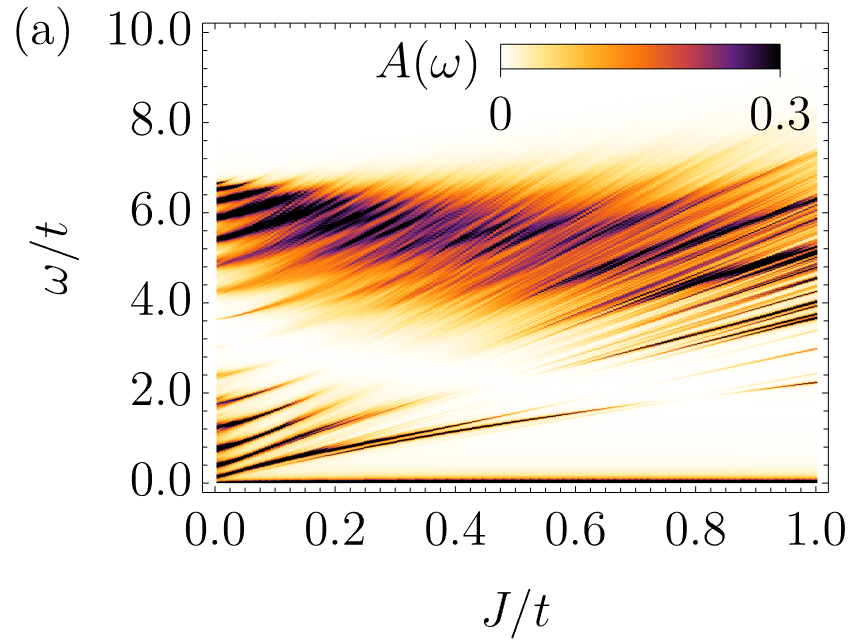
\includegraphics[width=0.49\columnwidth]
	{./figures/square/[0].png}
	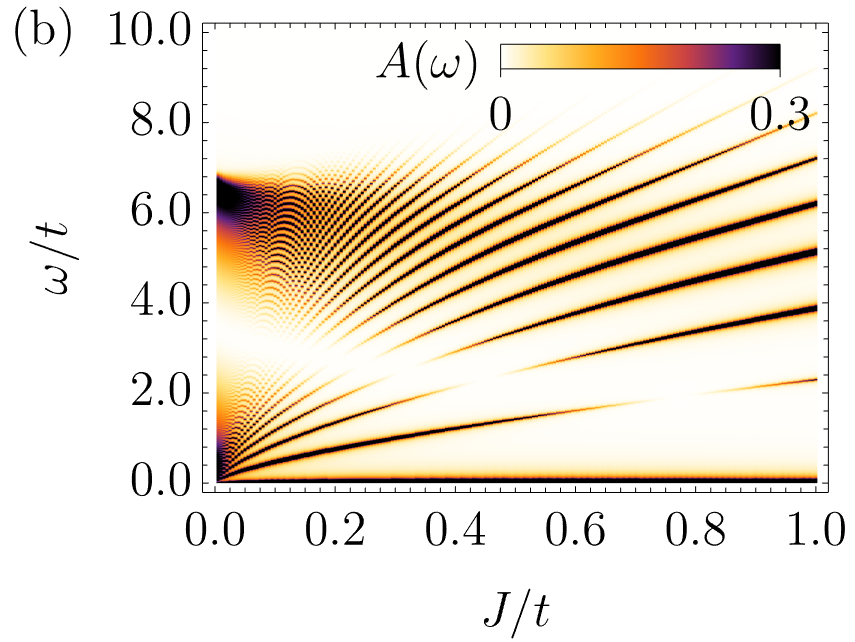
\includegraphics[width=0.49\columnwidth]
	{./figures/bethe/[0].png}
	\caption{
		Spectral function $A(\omega)$ of a singe hole with rotational degrees of freedom calculated within self-avoiding walks approximation (with interactions included), (a) on the square lattice and (b) on the Bethe lattice. Coupling constant $J=0.4t$, $m_4 = 0$.
	}\label{fig:rot_0}
\end{figure}

Let us start with $m_4 \equiv m^{(1)} = 0$ case. When we compare spactral functions in Fig.~\ref{fig:rot_0_no_mag} and Fig.~\ref{fig:rot_0} with their counterparts witout rotations, Fig.~\ref{fig:no_rot_no_mag} and Fig.~\ref{fig:no_rot} respectively, we can see the same set of peaks. The only qualitative difference between these spectral functions is a missing weight in the middle of the spectrum for the cases with rotational degree of freedom. Rotational degree of freedom is necessary but not sufficient condition for this effect to appear. We will cover this later in more details. Due to summation constraint missing weight in the middle makes the peaks more pronouced everywhere else. Nevertheless, spectral functions for $m_4 = 0$ do not provide any additional information over spectral functions without rotations.

\begin{figure}[ht!]
	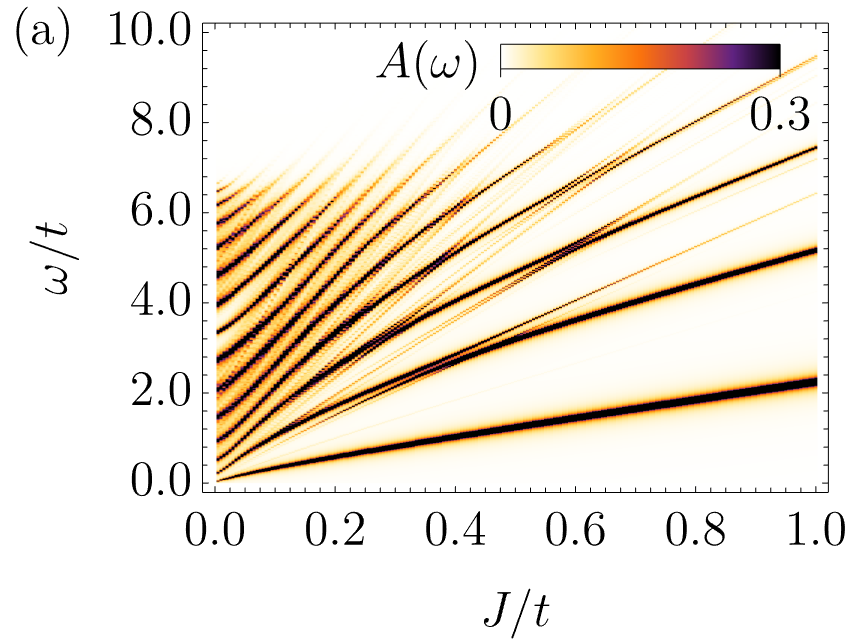
\includegraphics[width=0.49\columnwidth]
	{./figures/square/[1]_noint.png}
	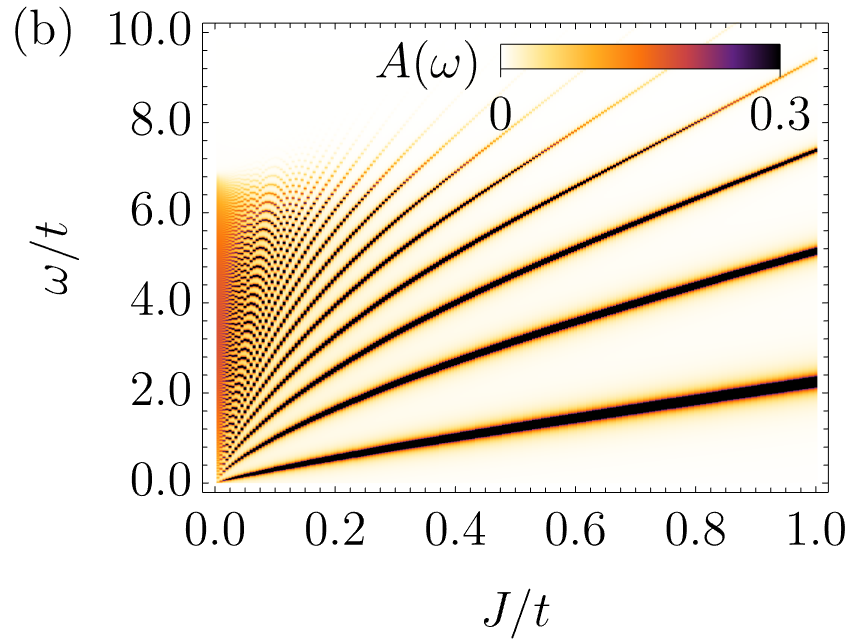
\includegraphics[width=0.49\columnwidth]
	{./figures/bethe/[1]_noint.png}
	\caption{
		Spectral function $A(\omega)$ of a singe hole with rotational degrees of freedom calculated within self-avoiding walks approximation without interactions, (a) on the square lattice and (b) on the Bethe lattice. Coupling constant $J=0.4t$, $m_4 = 1$.
	}\label{fig:rot_1_no_mag}
\end{figure}

\begin{figure}[ht!]
	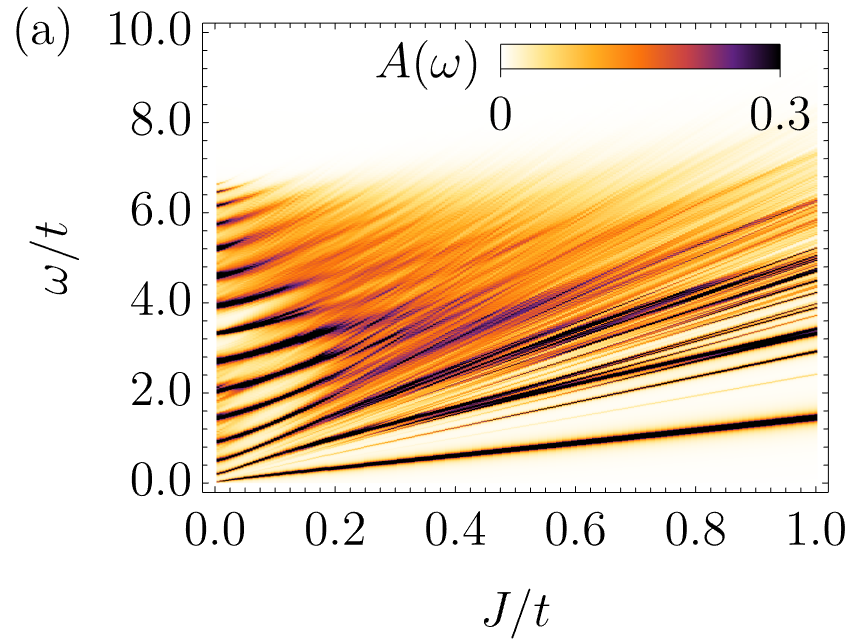
\includegraphics[width=0.49\columnwidth]
	{./figures/square/[1].png}
	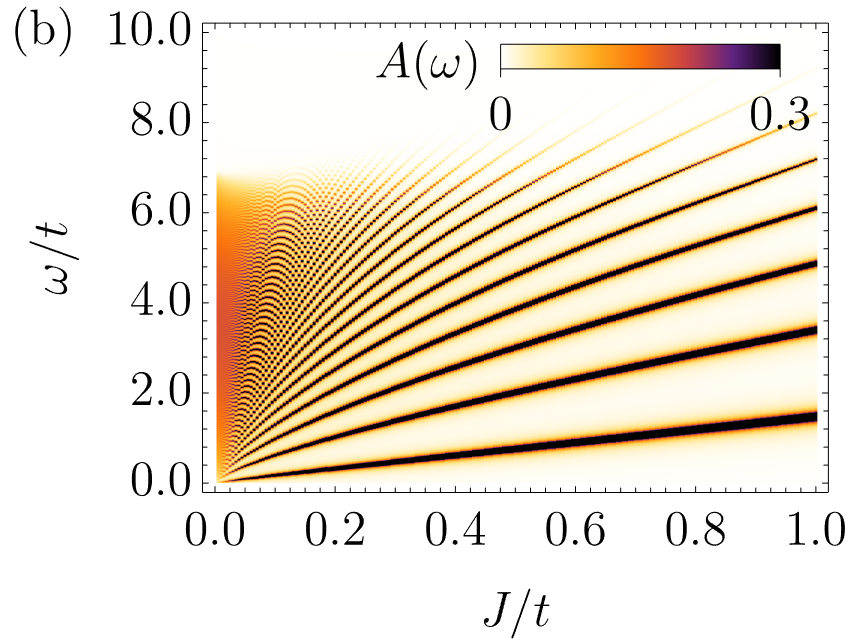
\includegraphics[width=0.49\columnwidth]
	{./figures/bethe/[1].png}
	\caption{
		Spectral function $A(\omega)$ of a singe hole with rotational degrees of freedom calculated within self-avoiding walks approximation (with interactions included), (a) on the square lattice and (b) on the Bethe lattice. Coupling constant $J=0.4t$, $m_4 = 1$.
	}\label{fig:rot_1}
\end{figure}

Next we will analyze the case of $m_4 = 1,2,3$. We can see that the ground state is not visible in these cases -- there is no peak at energy 0 in Fig.~\ref{fig:rot_1_no_mag} nor in Fig.~\ref{fig:rot_1}. Actually, at least for the Bethe lattice case, we can for sure say that none of the peaks visible in previous spectra is present in spectra with $m_4 = 1$. In fact ARPES measurement (corresponding to spectral function without rotations) measures only vibrational modes of the introduced hole. Thus some of the eigenstates of the system cannot be seen by this method. It is directly visible in Fig.~\ref{fig:rot_1_no_mag} and Fig.~\ref{fig:rot_1}, where the hole has nonzero angular momentum, which leads to the compeletely different set of peaks in the spectrum.

Not only the peaks are at different positions compared to previous spectra but also they behave differently when $J/t$ varies. We can clearly see that lowest peak in Fig.~\ref{fig:rot_1_no_mag} and Fig.~\ref{fig:rot_1} both with and without magnon interactios is linear in $J/t$. Higher energy peaks seem to have additional non-linear component but they are also close to linear dependence, especially for large $J/t$. On the other hand, there is no missing weight in the middle of the spectra, despite having rotational degree of freedom. Thus one can see that rotations are not sufficient to create the gap in spectrum by redistributing the weigth to lower and higher energies.

\subsection{\label{sec:results:two_rot}Spectral functions with two rotations}

Last set of results concerns a spectral functions of a hole with two rotational degrees of freedom. It corresponds to creating a hole in a given site and then propagating it twice (without returning), i.e. to next nearest sites. Each time the hole is propagated it acquires phase factor dependent on the direction of propagation.
\begin{equation}
	R_{\sigma,M_2}(0) \ket{0_\sigma} = \sum_{\substack{\xi_1 \in D \\ \xi_2 \in D\setminus\{\xi_1'\}}} e^{-i m^{(1)} \phi_{\xi_1}} e^{-i m^{(2)} \phi_{\xi_1 \xi_2}} \ket{\xi_1 \xi_2},
\end{equation}
where $D = \{E,N,W,S\}$ and $\xi_1'$ is direction opposite to $\xi_1$. Again $\phi_{\xi_1} \in \{\frac{n\pi}{2}\}_{n\in0...3}$ but $\phi_{\xi_1 \xi_2} \in \{\frac{n\pi}{3}\}_{n\in0...2}$ since there are 3 possible routes to propagate the hole futher (i.e. without returning). Similarily $m_4 \equiv m^{(1)} \in \{0,...,3\}$ and $m_3 \equiv m^{(2)} \in \{0,1,2\}$. For details on definition of $\phi_{\xi_1 \xi_2}$ have a look at the Appendix~\ref{sec:appendix:phases}. 

\begin{figure}[ht!]
	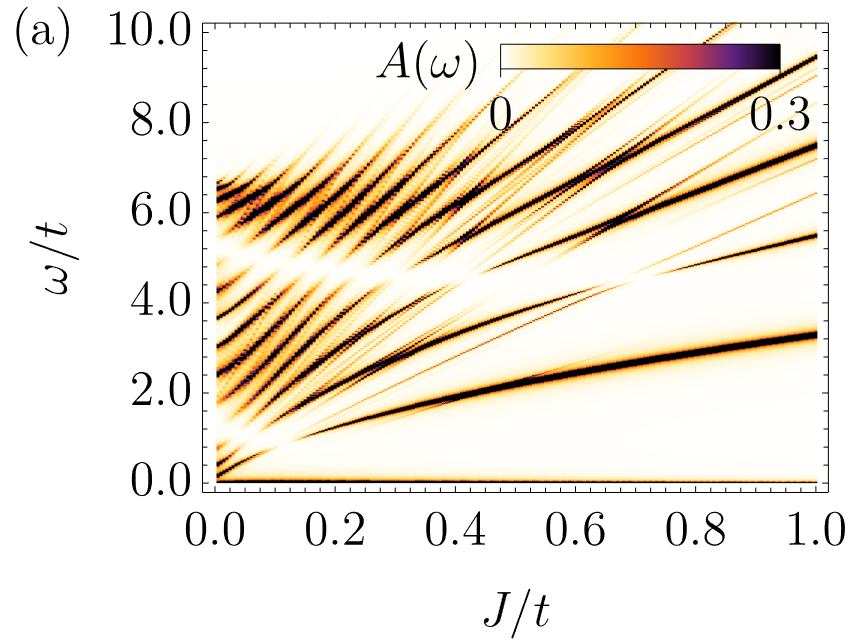
\includegraphics[width=0.49\columnwidth]
	{./figures/square/[0, 0]_noint.png}
	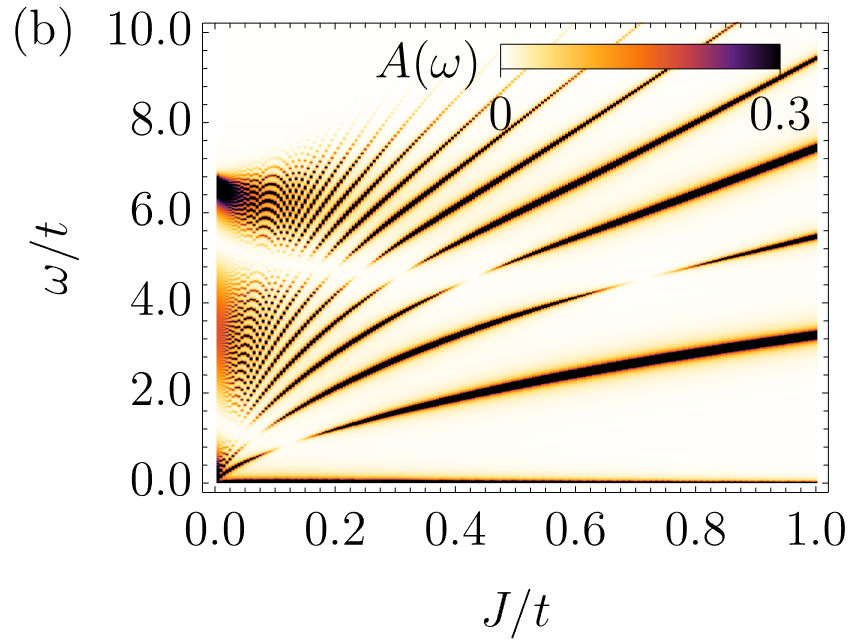
\includegraphics[width=0.49\columnwidth]
	{./figures/bethe/[0, 0]_noint.png}
	\caption{
		Spectral function $A(\omega)$ of a singe hole with rotational degrees of freedom calculated within self-avoiding walks approximation without interactions, (a) on the square lattice and (b) on the Bethe lattice. Coupling constant $J=0.4t$, $m_4 = 0$, $m_3 = 0$.
	}\label{fig:rot_00_no_mag}
\end{figure}

\begin{figure}[ht!]
	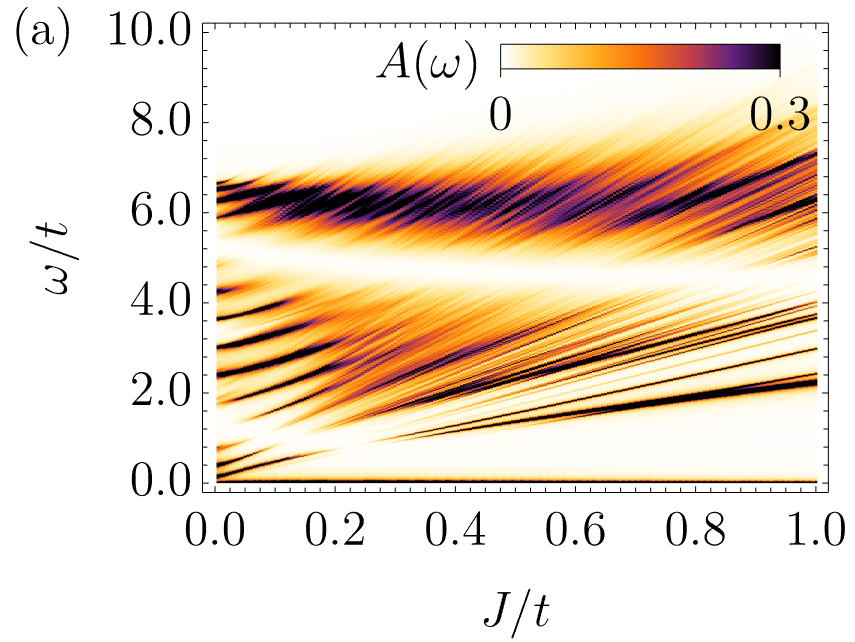
\includegraphics[width=0.49\columnwidth]
	{./figures/square/[0, 0].png}
	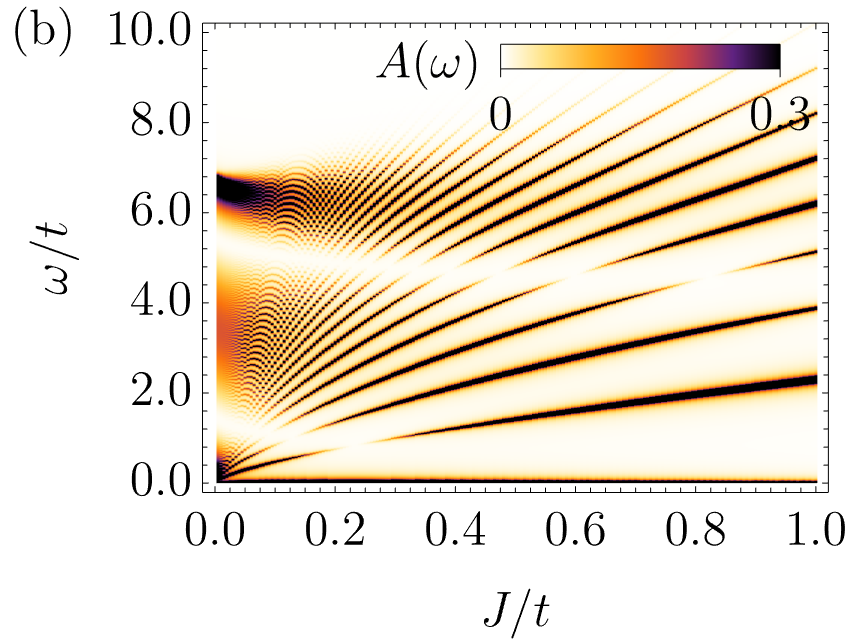
\includegraphics[width=0.49\columnwidth]
	{./figures/bethe/[0, 0].png}
	\caption{
		Spectral function $A(\omega)$ of a singe hole with rotational degrees of freedom calculated within self-avoiding walks approximation (with interactions included), (a) on the square lattice and (b) on the Bethe lattice. Coupling constant $J=0.4t$, $m_4 = 0$, $m_3 = 0$.
	}\label{fig:rot_00}
\end{figure}

We start with the case $(m_4,m_3) = (0,0)$, i.e. hole does not acquire any angular momentum in neither of the moves. We can clearly see that the corresponding spectral functions without magnon-magnon interactions presented in Fig.~\ref{fig:rot_00_no_mag} are qulitatively similar to those in Fig.~\ref{fig:no_rot_no_mag} and Fig.~\ref{fig:rot_0_no_mag}. The only difference is that now there are 2 regions where the weight of the peaks is washed away. But all the peaks are in exactly same positions in all mentioned figures. The same applies to the cases with magnon magnon interactions (cf. Fig.~\ref{fig:rot_00}, Fig.~\ref{fig:no_rot} and Fig.~\ref{fig:rot_0}).

\begin{figure}[ht!]
	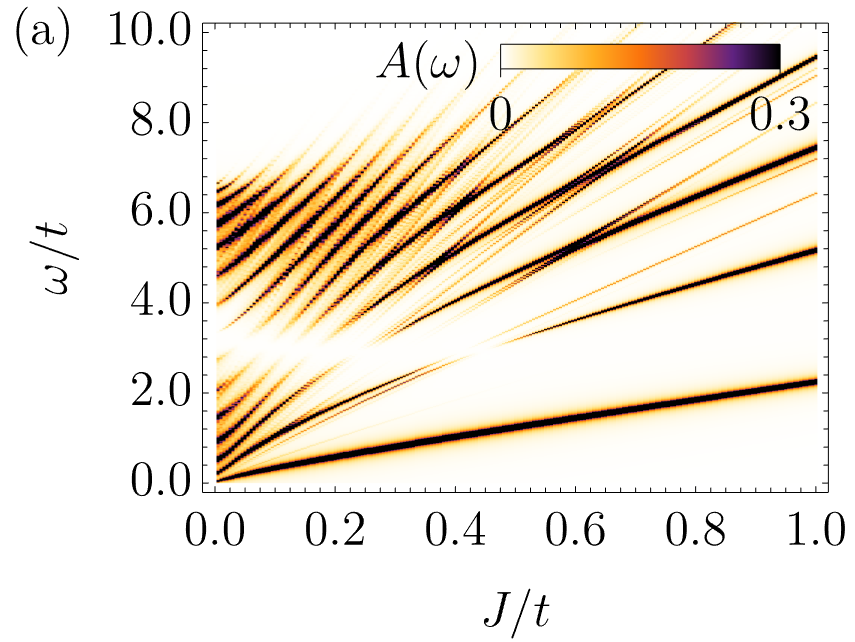
\includegraphics[width=0.49\columnwidth]
	{./figures/square/[1, 0]_noint.png}
	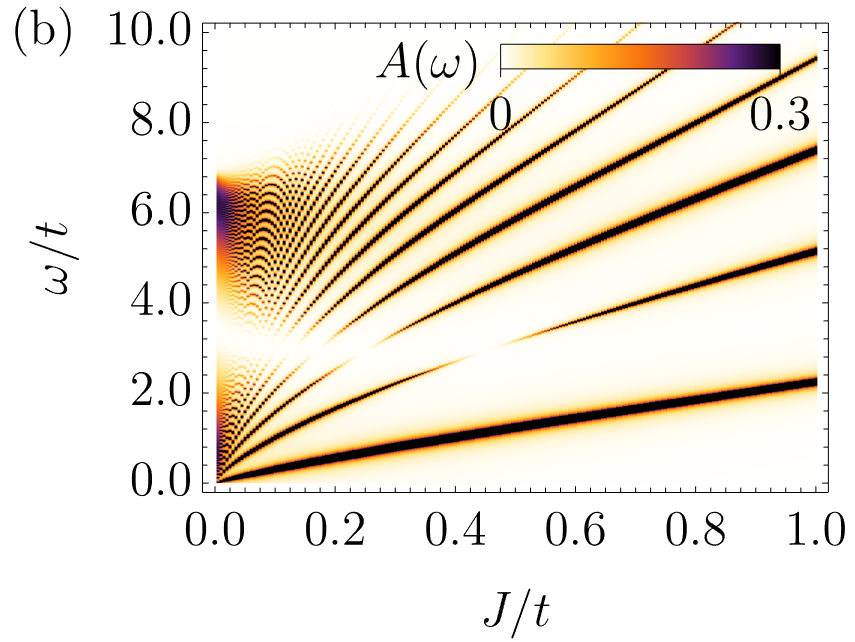
\includegraphics[width=0.49\columnwidth]
	{./figures/bethe/[1, 0]_noint.png}
	\caption{
		Spectral function $A(\omega)$ of a singe hole with rotational degrees of freedom calculated within self-avoiding walks approximation without interactions, (a) on the square lattice and (b) on the Bethe lattice. Coupling constant $J=0.4t$, $m_4 = 1$, $m_3 = 0$.
	}\label{fig:rot_10_no_mag}
\end{figure}

\begin{figure}[ht!]
	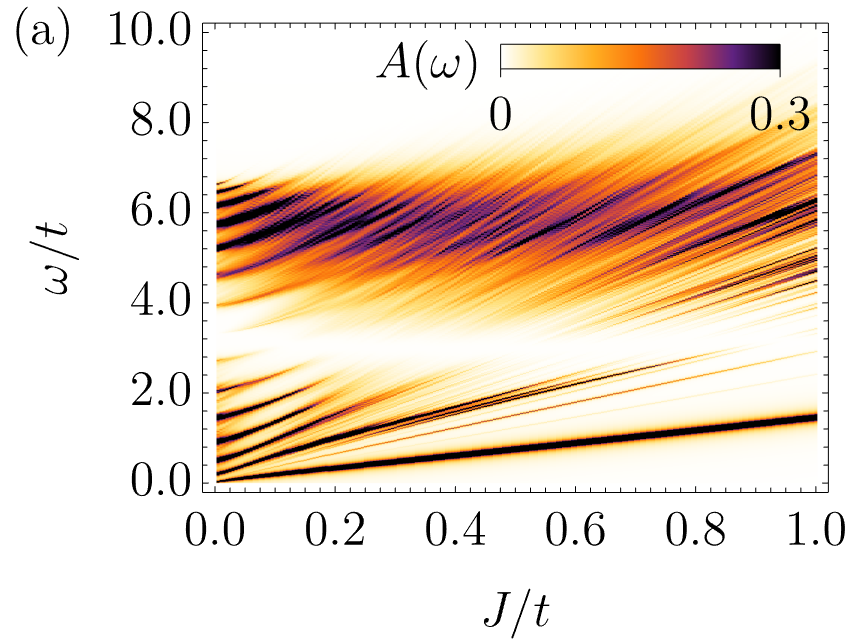
\includegraphics[width=0.49\columnwidth]
	{./figures/square/[1, 0].png}
	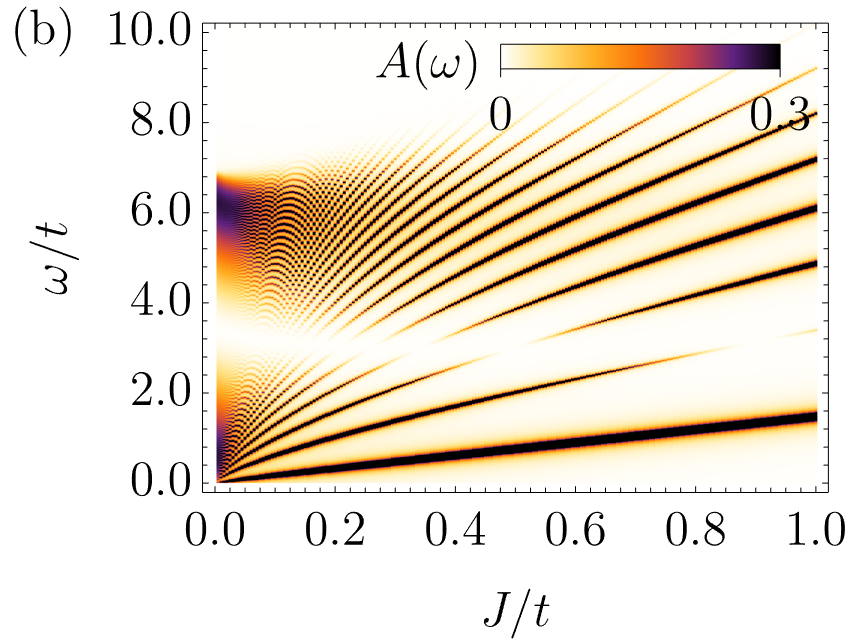
\includegraphics[width=0.49\columnwidth]
	{./figures/bethe/[1, 0].png}
	\caption{
		Spectral function $A(\omega)$ of a singe hole with rotational degrees of freedom calculated within self-avoiding walks approximation (with interactions included), (a) on the square lattice and (b) on the Bethe lattice. Coupling constant $J=0.4t$, $m_4 = 1$, $m_3 = 0$.
	}\label{fig:rot_10}
\end{figure}

Next we study the case with $(m_4, m_3) = (1,0)$. This case is more interresting. On the qualitative level, i.e. when it comes to the set of peaks present in the spectral function, the spectral functions presented in Fig.~\ref{fig:rot_10_no_mag} are equivalent to previous case of single rotation $m_4 = 1$, see Fig.~\ref{fig:rot_1_no_mag}. The same applies when we introduce magnon interactions, cf. Fig.~\ref{fig:rot_10} with Fig.~\ref{fig:rot_1}. On top of this, the fact that now we have $m_3 = 0$ introduces a region where the weight of peaks is removed. We could see the same behavior with $m_4 = 0$ in spectral functions with single rotation (see Fig.~\ref{fig:rot_0_no_mag}, Fig.~\ref{fig:rot_0}).

\begin{figure}[ht!]
	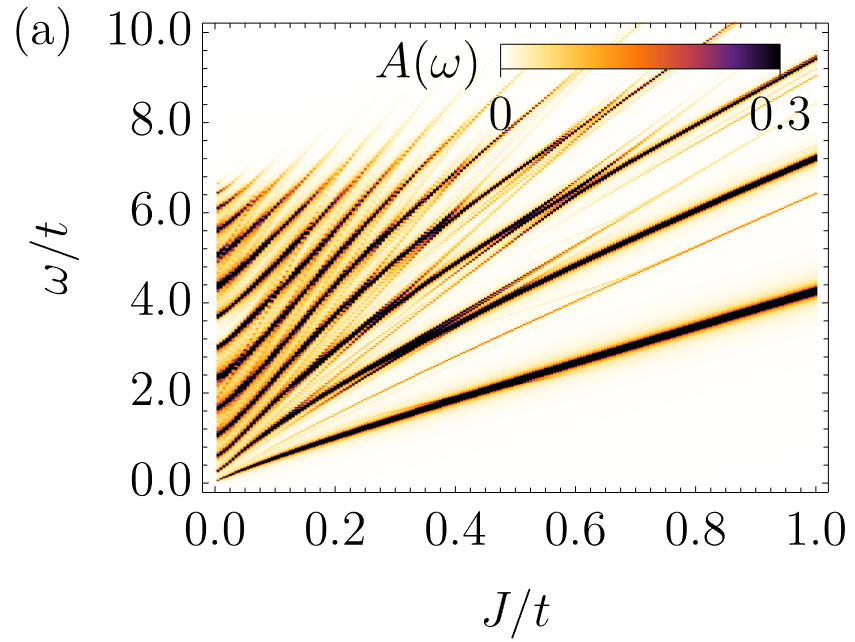
\includegraphics[width=0.49\columnwidth]
	{./figures/square/[0, 1]_noint.png}
	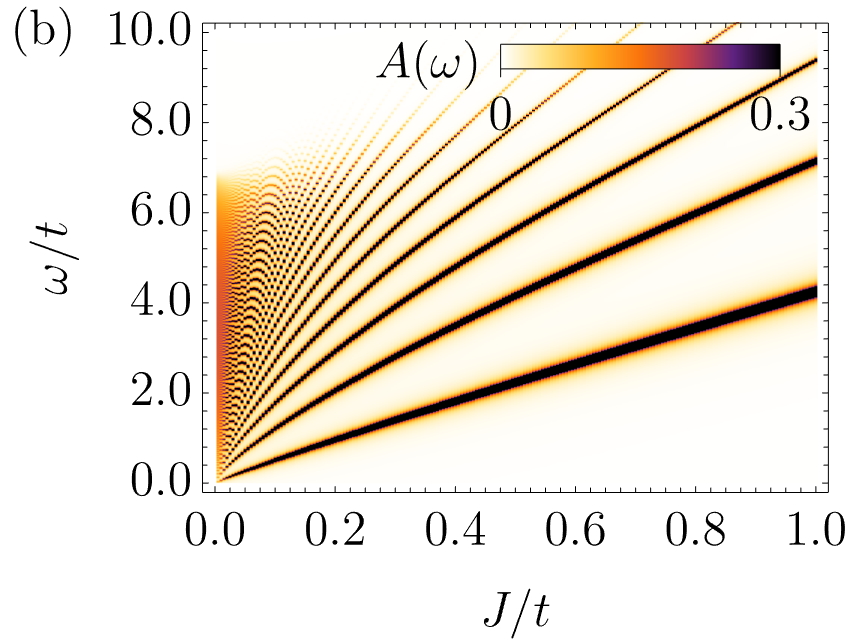
\includegraphics[width=0.49\columnwidth]
	{./figures/bethe/[0, 1]_noint.png}
	\caption{
		Spectral function $A(\omega)$ of a singe hole with rotational degrees of freedom calculated within self-avoiding walks approximation without interactions, (a) on the square lattice and (b) on the Bethe lattice. Coupling constant $J=0.4t$, $m_4 = 0$, $m_3 = 1$.
	}\label{fig:rot_01_no_mag}
\end{figure}

\begin{figure}[ht!]
	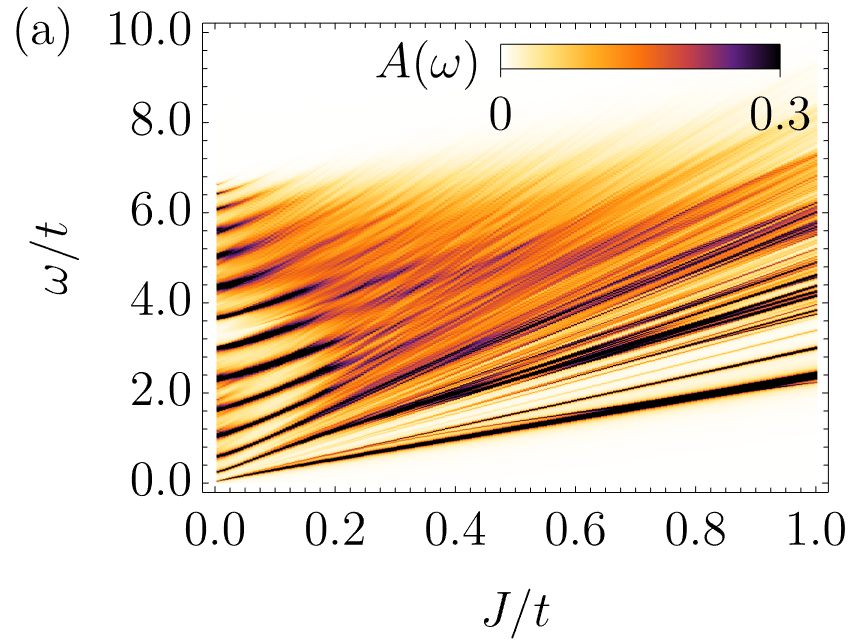
\includegraphics[width=0.49\columnwidth]
	{./figures/square/[0, 1].png}
	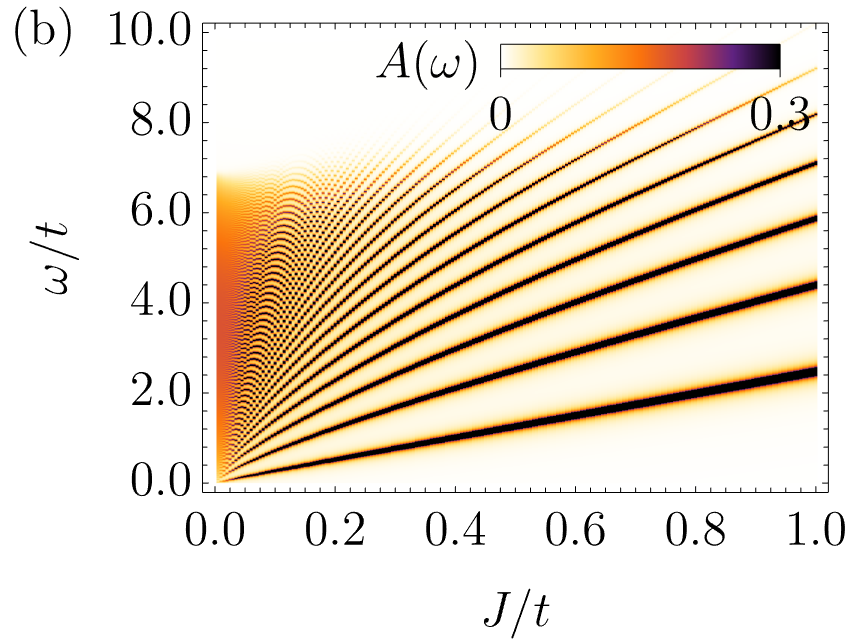
\includegraphics[width=0.49\columnwidth]
	{./figures/bethe/[0, 1].png}
	\caption{
		Spectral function $A(\omega)$ of a singe hole with rotational degrees of freedom calculated within self-avoiding walks approximation (with interactions included), (a) on the square lattice and (b) on the Bethe lattice. Coupling constant $J=0.4t$, $m_4 = 0$, $m_3 = 1$.
	}\label{fig:rot_01}
\end{figure}

Now let swap the values of phase factor and analyze the case of $(m_4,m_3) = (0,1)$. Corresponding spectral functions ommiting and including magnon interactions are presented in Fig.~\ref{fig:rot_01_no_mag} and Fig.~\ref{fig:rot_01} respectively. We can see there is no region of suppresed wieght despite $m_4 = 0$. Combining this with previous results we can conjecture that number of regions with dumped weight is equal to the number of consequent jumps of the hole without acquiring the angular momentum counted from the last move to the first move. 

The set of peaks present in Fig.~\ref{fig:rot_01_no_mag} and Fig.~\ref{fig:rot_01} is different from previous results. But on qualitative level this case is similar to case with single rotation and $m_4 = 1$, (cf. Fig.~\ref{fig:rot_1_no_mag} and Fig.~\ref{fig:rot_1}). Specifically, there is no peak at the ground state energy and the first visible peak is linear in $J/t$. Higher energy peaks are almost linear, especially for large $J/t$.

\begin{figure}[ht!]
	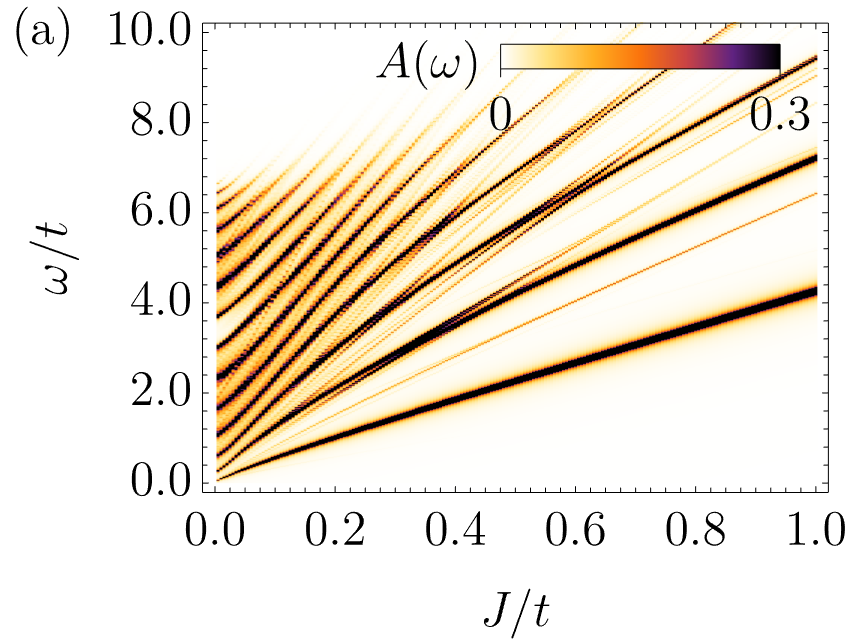
\includegraphics[width=0.49\columnwidth]
	{./figures/square/[1, 1]_noint.png}
	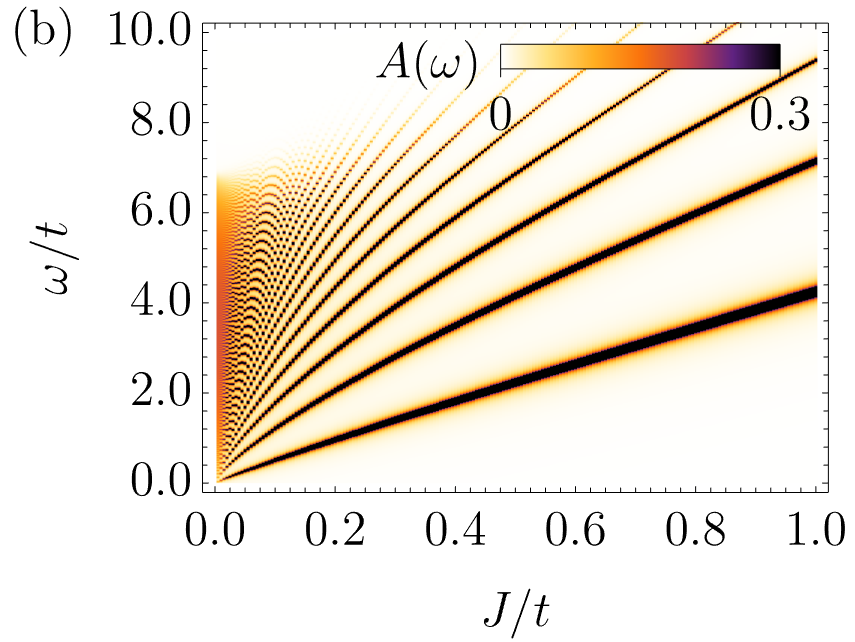
\includegraphics[width=0.49\columnwidth]
	{./figures/bethe/[1, 1]_noint.png}
	\caption{
		Spectral function $A(\omega)$ of a singe hole with rotational degrees of freedom calculated within self-avoiding walks approximation without interactions, (a) on the square lattice and (b) on the Bethe lattice. Coupling constant $J=0.4t$, $m_4 = 1$, $m_3 = 1$.
	}\label{fig:rot_11_no_mag}
\end{figure}

\begin{figure}[ht!]
	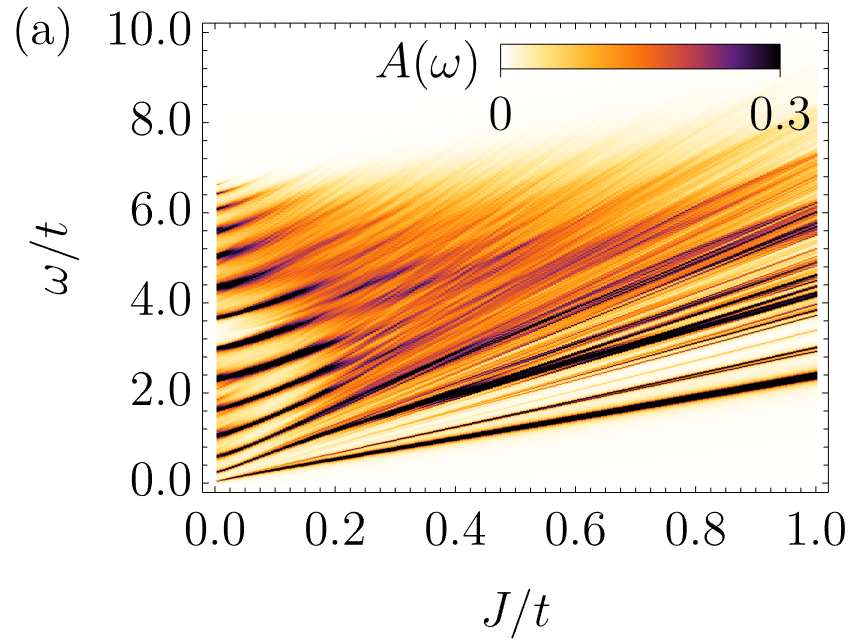
\includegraphics[width=0.49\columnwidth]
	{./figures/square/[1, 1].png}
	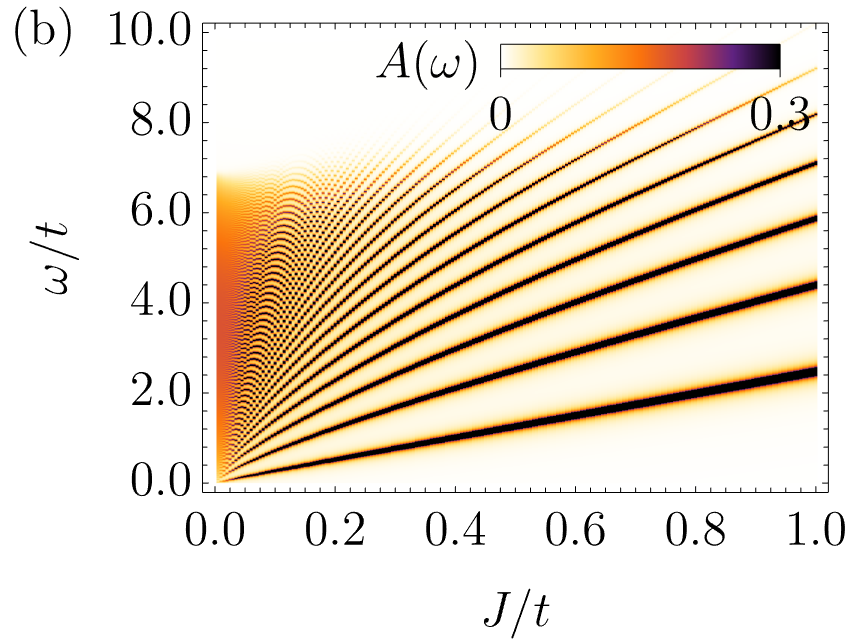
\includegraphics[width=0.49\columnwidth]
	{./figures/bethe/[1, 1].png}
	\caption{
		Spectral function $A(\omega)$ of a singe hole with rotational degrees of freedom calculated within self-avoiding walks approximation (with interactions included), (a) on the square lattice and (b) on the Bethe lattice. Coupling constant $J=0.4t$, $m_4 = 1$, $m_3 = 1$.
	}\label{fig:rot_11}
\end{figure}

The last presented set of figures concerns $(m_4,m_3) = (1,1)$. We can see that result for the Bethe lattice (Fig.~\ref{fig:rot_11_no_mag}b and Fig.~\ref{fig:rot_11}b) looks the same as in the discussed in previous paragraphs case of $m_4 = 0$ (see Fig.~\ref{fig:rot_01_no_mag}b and Fig.~\ref{fig:rot_01}b). Similarily, results on square lattice seem to be the same, but in this case there are small differences, barely visible in the spectrum. Compared to $m_4 = 0$ case, very faint additional peaks appear, even without magnon interactions (cf. Fig.~\ref{fig:rot_11_no_mag}a and Fig.~\ref{fig:rot_01_no_mag}a). When magnon interactions are included these changes are more pronounced (cf. Fig.~\ref{fig:rot_11}a and Fig.~\ref{fig:rot_01}a). Such behaviour suggest that this effect originates from existence of tangential paths on the square lattice. Nevertheless, it is rather negligible contribution to the overall shape of the spectrum.


\section{\label{sec:discussion}Discussion}

\section{\label{sec:conclusions}Conclusions}

\section*{\label{sec:acknowledgements}Acknowledgements}
We  kindly  acknowledge  support  by  the  (Polish)  National  Science  Centre  (NCN, Poland)  under  Projects  No. 2016/22/E/ST3/00560 (PW and KW), 2016/23/B/ST3/00839 (KW). The calculations were performed at the ICM cluster.


\appendix
\section{\label{sec:appendix:phases}Phase factors}
Let us define here phase factor $\mathcal{P}_{M_n}^{\eta',\eta}$. It depends on the two paths $\eta$ and $\eta'$ as well as on set of $n$ free parameters. For $n = 0$ and $n = 1$ the case is trivial and it was described in the Results: Sec.~\ref{sec:results:no_rot} and Sec.~\ref{sec:results:one_rot} respectively. In our investigation we have $n \leq 2$ so let us proceed by assuming $n = 2$. 
Then we can write,
\begin{equation}
	\mathcal{P}_{M_2}^{\xi_1' \xi_2', \xi_1 \xi_2} = e^{i\left(m_4\phi_{\xi_1'} + m_3\phi_{\xi_1' \xi_2'}\right) - i\left(m_4\phi_{\xi_1} + m_3\phi_{\xi_1 \xi_2}\right)},
\end{equation}
where $M_2 = (m_4, m_3)$ and $m_k \in \{0,...,k-1\}$. The only difficulty here is the relation of phases $\phi_\xi$ to the paths opf the hole -- there are multiple ways to define it. Here we describe our choice. We for the first move set in standard way $\phi_{\xi_1} = \frac{n\pi}{4}$, where
\begin{itemize}	
	\item $n = 0$ if $\xi_1 = E$,
	\item $n = 1$ if $\xi_1 = N$,
	\item $n = 2$ if $\xi_1 = W$,
	\item $n = 3$ if $\xi_1 = S$.
\end{itemize}
The phase of the second move depends of the second move and on the first move as well. In general, $\phi_{\xi_1 \xi_2} = \frac{m\pi}{3}$, where for $\xi_1 = E$ we have,
\begin{itemize}	
	\item $m = 0$ if $\xi_2 = E$,
	\item $m = 1$ if $\xi_2 = N$,
	\item $m = 2$ if $\xi_2 = S$.
\end{itemize}
Other paths have the above set of 3 values rotated accordingly to the direction of the first move, such that $m = 0$ correspondts to $\xi_2 = \xi_1$. E.g. for $\xi_1 = N$ we have,
\begin{itemize}	
	\item $m = 0$ if $\xi_2 = N$,
	\item $m = 1$ if $\xi_2 = W$,
	\item $m = 2$ if $\xi_2 = E$.
\end{itemize}
% For the graphical interpretation see a graph below.
% \begin{center}
%     \begin{tikzpicture}[
%     roundnode/.style={circle, draw=black!60, fill=blue!10, very thick, minimum size=0.1}
%     ]
%         %Nodes
%         \node[roundnode]    
%             (m0)                    {};
%         \node[roundnode]    
%             (mE)     [right=of m0]   	{$n = 0$};
% 		\node[roundnode]    
%             (mN)     [above=of m0]   	{$n = 1$};
% 		\node[roundnode]    
%             (mW)     [left=of m0]    	{$n = 2$};
% 		\node[roundnode]    
%             (mS)     [below=of m0]   	{$n = 3$};

%         \node[roundnode]    
%             (mEE)    [right=of mE]   	{$m = 0$};
%         \node[roundnode]    
%             (mEN)    [above=of mE]   	{$m = 1$};
% 		\node[roundnode]    
%             (mES)    [below=of mE]   	{$m = 2$};

% 		\node[roundnode]    
%             (mNN)    [above=of mN]   	{$m = 0$};
%         \node[roundnode]    
%             (mNW)    [left=of mN]   	{$m = 1$};
% 		\node[roundnode]    
%             (mNE)    [right=of mN]   	{$m = 2$};
        
%         %Lines
%         \draw[-, >=stealth, draw=black!60, very thick] 
%             (m0.east) -- (mE.west);
% 		\draw[-, >=stealth, draw=black!60, very thick] 
%             (m0.north) -- (mN.south);
% 		\draw[-, >=stealth, draw=black!60, very thick] 
%             (m0.west) -- (mW.east);
% 		\draw[-, >=stealth, draw=black!60, very thick] 
%             (m0.south) -- (mS.north);

% 		\draw[-, >=stealth, draw=black!60, very thick] 
%             (mE.east) -- (mEE.west);
% 		\draw[-, >=stealth, draw=black!60, very thick] 
%             (mE.north) -- (mEN.south);
% 		\draw[-, >=stealth, draw=black!60, very thick] 
%             (mE.south) -- (mES.north);
%     \end{tikzpicture}
% \end{center}

\section{\label{sec:appendix:diagrams}Diagrams}

To grasp the essence of the equation \eqref{eq:GFcoef} for $G_{\eta', \eta}(\omega)$ it is instructive to express it through diagrams. To this end, let us formulate rules for creating the diagrams in terms of the introduced notation. 
\begin{enumerate}
    \item Diagram consists of nodes connected with single lines or double lines. Nodes correspond to states of the system, while lines represent the propagation of the hole. Single lines represent propagation distinct in the left $\bra{\eta'}$ and the right $\ket{\eta}$ states while double lines correspond to common parts of the path.
    \item Each node is labeled with its corresponding weight $\Gamma_{\eta}^{\mathcal{S}(\eta)}$, where $\eta$ is state of the system in moves notation.
    \item Single lines are denoted with $-t$ as they add a factor of $-t$ to the whole solution.
    \item Double line corresponding to move $\xi \in D$ and starting from the node denoted with $\Gamma_{\eta}^{\mathcal{S}(\eta)}$ is denoted with $\Gamma_{\eta}^{\mathcal{S}(\eta) \setminus \{\xi\}}$.
    \item Each line ends with arrow denoting direction of hole motion (i.e. order of operators $\xi_j \in D$) in the left and the right state.
\end{enumerate}

With the above, the local Greens function can be written as follows,
\begin{equation}
    G_{1,1}(\omega) = \frac{1}{\Gamma_1^{D}(\omega)},
\end{equation}
or expressed through the simplest diagram.
\begin{center}
	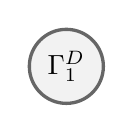
\begin{tikzpicture}[
	roundnode/.style={circle, draw=black!60, fill=black!5, very thick, minimum size=0.25}
	]
		%Nodes
		\node[roundnode]    
			(m0)                    {$\Gamma_1^{D}$};
			
	\end{tikzpicture} 
\end{center}
For the coefficient $G_{EE,EE}$ the diagram is as follows,
\begin{center}
    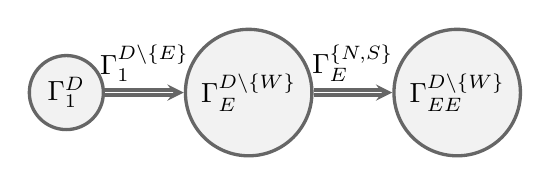
\begin{tikzpicture}[
    roundnode/.style={circle, draw=black!60, fill=black!5, very thick, minimum size=0.25}
    ]
        %Nodes
        \node[roundnode]    
            (m0)                    {$\Gamma_1^{D}$};
        \node[roundnode]    
            (mE)    [right=of m0]   {$\Gamma_E^{D \setminus \{W\}}$};
        \node[roundnode]    
            (mEE)    [right=of mE]   {$\Gamma_{EE}^{D \setminus \{W\}}$};
        
        %Lines
        \draw[->, >=stealth, draw=black!60, very thick, double] 
            (m0.east) -- node[above] {$\Gamma_1^{D \setminus \{E\}}$} (mE.west);
        \draw[->, >=stealth, draw=black!60, very thick, double] 
            (mE.east) -- node[above] {$\Gamma_E^{\{N,S\}}$} (mEE.west);
    \end{tikzpicture}
\end{center}
so we can read out the expression,
\begin{equation}
	G_{EE,EE}(\omega) = \frac{
	\left(
	\Gamma_1^{D \setminus \{E\}}
	-\frac{t^2}{\Gamma_E^{\{N,S\}}}
	\right)
	\Gamma_E^{\{N,S\}}
	}
	{
		\Gamma_1^{D}
		\Gamma_E^{D \setminus \{W\}}
		\Gamma_{EE}^{D \setminus \{W\}}
	}.
\end{equation}
Compare it with the Eq.~\eqref{eq:GFcoef}. Similarily for $G_{EN,EE}$,
\begin{center}
    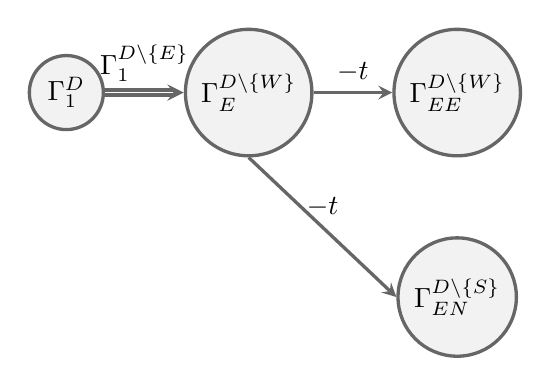
\begin{tikzpicture}[
    roundnode/.style={circle, draw=black!60, fill=black!5, very thick, minimum size=0.25}
    ]
        %Nodes
        \node[roundnode]    
            (m0)                    {$\Gamma_1^{D}$};
        \node[roundnode]    
            (mE)    [right=of m0]   {$\Gamma_E^{D \setminus \{W\}}$};
        \node[roundnode]    
            (mEE)    [right=of mE]   {$\Gamma_{EE}^{D \setminus \{W\}}$};
        \node[roundnode]    
            (mEN)    [below=of mEE]   {$\Gamma_{EN}^{D \setminus \{S\}}$};
        
        %Lines
        \draw[->, >=stealth, draw=black!60, very thick, double] 
            (m0.east) -- node[above] {$\Gamma_1^{D \setminus \{E\}}$} (mE.west);
        \draw[->, >=stealth, draw=black!60, very thick] 
            (mE.east) -- node[above] {$-t$} (mEE.west);
        \draw[->, >=stealth, draw=black!60, very thick] 
            (mE.south) -- node[above] {$-t$} (mEN.west);
    \end{tikzpicture}
\end{center}
we can read out the formula from its diagram,
\begin{equation}
	G_{EE,EN}(\omega) = \frac{
	t^2\Gamma_1^{D \setminus \{E\}}
	}
	{
		\Gamma_1^{D}
		\Gamma_E^{D \setminus \{W\}}
		\Gamma_{EE}^{D \setminus \{W\}}
		\Gamma_{EN}^{D \setminus \{S\}}
	}.
\end{equation}

Moreover, while performing the calculations one shall take the advantage of the symmetries of the system, e.g. $G_{EE,EE} = G_{NN,NN} = G_{WW,WW} = G_{SS,SS}$, to reduce the number of terms that have to be calculated to find Greens function with rotations.

\bibliographystyle{apsrev4-1}
\bibliography{rot}

\end{document}